\documentclass{article}
\usepackage[utf8]{inputenc}
\usepackage{subfiles}
\usepackage{amsmath}
\usepackage{pgfplots}
\usepackage{textcomp}
\usepackage{csquotes}
\pgfplotsset{compat=1.12}
\pgfplotsset{width=10cm}
\pgfplotsset{holdot/.style={color=blue,fill=white,only marks,mark=*}}
\pgfplotsset{dot/.style={color=blue,fill=blue,only marks,mark=*}}
\usepgfplotslibrary{groupplots}
%\usepgfplotslibrary{fillbetween}
\title{Noah's Guide to Calculus}
\author{Noah Stockwell}
\date{Summer 2016}
\begin{document}
\maketitle
\vspace{2in}
\begin{center}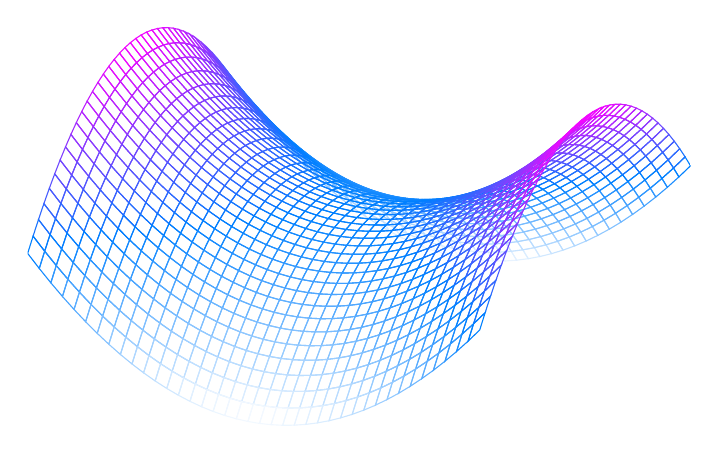
\begin{tikzpicture}\begin{axis}[hide axis,
xlabel=$x$,ylabel=$y$,colormap/cool, ]
\addplot3[domain=-3:3,mesh,samples=40]{x^2-y^2};
\end{axis}\end{tikzpicture}\end{center}
\newpage
\tableofcontents
\newpage

\section{Limits} \subfile{revisedsections/IntroToLimits}
\subsection{Types of Limits} \subfile{revisedsections/TypesOfLimits} 
\subsection{Directly Calculating Limits} \subfile{revisedsections/DirectlyCalculatingLimits}
\subsection{The Squeeze Theorem} \subfile{revisedsections/SqueezeTheorem}
\subsection{Relative Magnitudes} \subfile{revisedsections/LimitRelativeMagnitudes}

\section{Derivatives} \subfile{revisedsections/IntroToDerivatives}
\subsection{Difference Quotient} \subfile{revisedsections/DifferenceQuotient}
\subsection{Estimating Derivatives}\subfile{revisedsections/EstimatingDerivatives}
\subsection{Rules} \subfile{revisedsections/DerivativeRules}
\subsection{Implicit Differentiation}\subfile{revisedsections/ImplicitDifferentiation}
\subsection{Maxima and Minima} \subfile{revisedsections/MaxAndMin}
\subsection{Concavity} \subfile{revisedsections/Concavity}
\subsection{Graphical Relations} \subfile{revisedsections/DerivativeGraphs}
\subsection{Relationship with Continuity} \subfile{revisedsections/DerivativesAndContinuity}

\section{Applications of Derivatives}
\subsection{Units}\subfile{revisedsections/DerivativeUnits}
\subsection{Instantaneous Rate of Change}\subfile{revisedsections/InstantaneousRateOfChange}
\subsection{Tangent Line Approximations}\subfile{revisedsections/TangentLineApproximations}
\subsection{Physics}\subfile{revisedsections/DerivativePhysics}
\subsection{Related Rates}\subfile{revisedsections/DerivativeRelatedRates}
\subsection{Optimization}\subfile{revisedsections/Optimization}
\subsection{Differential Equations}\subfile{revisedsections/DifferentialEquations}
\subsection{Slope Fields}\subfile{revisedsections/SlopeFields}
\subsection{Mean Value Theorem}\subfile{revisedsections/MeanValueTheorem}
\subsection{L'h\^{o}pital's Rule}\subfile{revisedsections/LhospitalsRule}

\end{document}
